\subsubsection{Анализ методов численного дифференцирования}

Использование методов численного дифференцирования, основанных на регуляризации полной вариации, осложняется наличием у этих методов параметров. Оба метода имеют параметр, отвечающий за степень регуляризации, второй метод, будучи итеративным, также содержит ограничение на число итераций. Поэтому в данном пункте будут проанализированы эти методы, проведено сравнение с методом конечных разностей и выявлены закономерности влияния параметров на конечный результат.

Параметр $\alpha$ --- коэффициент регуляризации --- несет одинаковую функцию в обоих методах: определяет насколько сильно будет подвергаться регуляризации процесс дифференцирования. Так как речь идет о регуляризации полной вариации, его влияние на производную очевидно: при увеличении $\alpha$, полная вариация производной будет уменьшаться, приводя к \enquote{уплощению} графика, до тех пор, пока он не выродится в прямую линию. Это подтверждает пример с дифференцированием синусоиды (без добавочного шума) на рисунке~\ref{fig:dif:alpha}.

\begin{figure}
\includegraphics[width=0.9\textwidth]{dif/alpha}
\caption{Результаты дифференцирования при различных значениях параметра $\alpha$}
\label{fig:dif:alpha}
\end{figure}

Для итеративного метода параметром также является число итераций. Итеративный процесс сходится к некоторому стационарному состоянию, пример значений производной той же самой синусоиды (уровень шума --- $0.05$) на разных итерациях показан на рисунке~\ref{fig:dif:max_iter}. Так как в этом случае речь идет о полной вариации полученной производной, на графиках видно увеличение ступенчатости --- количества и размеров областей с постоянными значениями, которые имеют нулевую вариацию.

\begin{figure}
\includegraphics[width=0.9\textwidth]{dif/max_iter}
\caption{Результаты дифференцирования на различных итерациях}
\label{fig:dif:max_iter}
\end{figure}

Рассмотрим подробный анализ обоих методов для трех тестовых функций.

\paragraph{Простая функция с непрерывной производной}

В качестве простой функции с непрерывной производной выбрана функция $sin(x)$ на отрезке $[0, 10]$. Она представлена на рисунке~\ref{fig:dif:sin}.

\begin{figure}
\includegraphics[width=0.5\textwidth]{dif/sin}
\caption{Функция $sin(x)$}
\label{fig:dif:sin}
\end{figure}

Для каждого метода рассмотрим среднюю абсолютную ошибку между результатом дифференцирования и точной производной для:
\begin{itemize}
\item различных разбиений отрезка и фиксированных параметрах,
\item различных уровней шума и фиксированных параметрах,
\item различных величин одного из параметров,
\item комбинаций уровней шума и значений параметра.
\end{itemize}

На рисунке~\ref{fig:dif:sin_fast_tvr} представлено тестирование первого метода.

\begin{figure}
\includegraphics[width=\textwidth]{dif/sin_fast_tvr}
\caption{Тестирование первого метода дифференцирования}
\label{fig:dif:sin_fast_tvr}
\end{figure}

Увеличение разбиения ожидаемо приводит к увеличению точности. Увеличение уровня шума при неизменных параметрах --- к ухудшению результата, возникает задача подбора параметров. Самый большой интерес представляют результаты комбинаций уровня шума и коэффициента регуляризации (серой пунктирной линией обозначена траектория с минимальной ошибкой): большие значения приводят к плохим результатам из-за сильного сглаживания производной, в остальном, можно сказать, что коэффициент регуляризации должен иметь схожий порядок с уровнем шума.

Тестирование второго метода, показанного на рисунке~\ref{fig:dif:sin_tvr}, приводит к схожим результатам. Отдельно стоит отметить влияние на результат числа итераций. При низком уровне шума оно практически не влияет, при больших --- ухудшает результат. Оптимальное число итераций --- 2.

\begin{figure}
\includegraphics[width=\textwidth]{dif/sin_tvr}
\caption{Тестирование второго метода дифференцирования}
\label{fig:dif:sin_tvr}
\end{figure}

Таким образом можно подобрать параметры для приемлемого дифференцирования данных с различным уровнем шума. Это показано на рисунке~\ref{fig:dif:sin_test}. Столбцы соответствуют различным уровням шума (первый столбец --- точные значения функции и производной), строки --- зашумленным данным, методу конечных разностей, первого и второму методам регуляризации полной вариации соответственно. Очень хорошо видно поведение метода конечных разностей, который перестает справляться с задачей при малейшем шуме.

\begin{figure}
\includegraphics[width=\textwidth]{dif/sin_test}
\caption{Дифференцирование данных с различным уровнем шума}
\label{fig:dif:sin_test}
\end{figure}

\paragraph{Простая функция с разрывной производной}

В качестве функции с разрывной производной выбрана функция модуля $|x|$ на отрезке $[-1, 1]$. Она изображена на рисунке~\ref{fig:dif:abs}.

\begin{figure}
\includegraphics[width=0.5\textwidth]{dif/abs}
\caption{Функция $|x|$}
\label{fig:dif:abs}
\end{figure}

На рисунках~\ref{fig:dif:abs_fast_tvr},~\ref{fig:dif:abs_tvr} представлены результаты тестирования методов. В целом наблюдается довольно похожая картина, однако, более сложный характер функции несколько осложняет дифференцирование. Соотношение между уровнем шума и коэффициентом регуляризации тоже несколько поменялось, теперь коэффициент должен быть на один-два порядка меньше.

\begin{figure}
\includegraphics[width=0.9\textwidth]{dif/abs_fast_tvr}
\caption{Тестирование первого метода дифференцирования}
\label{fig:dif:abs_fast_tvr}
\end{figure}

\begin{figure}
\includegraphics[width=0.9\textwidth]{dif/abs_tvr}
\caption{Тестирование второго метода дифференцирования}
\label{fig:dif:abs_tvr}
\end{figure}

На рисунке~\ref{fig:dif:abs_test} показаны результаты дифференцирования функции с различным уровнем шума. Заметно сглаживание места разрыва с усилением шума, однако, даже когда исходная функция слабо различима, основной характер производной все еще хорошо заметен.

\begin{figure}
\includegraphics[width=\textwidth]{dif/abs_test}
\caption{Дифференцирование данных с различным уровнем шума}
\label{fig:dif:abs_test}
\end{figure}

\paragraph{Сложная функция с непрерывной производной}

В качестве более сложной функции чем синус, но все еще с непрерывной производной, выбран аттрактор Лоренца --- решение системы Лоренца. Аттрактор изображен на рисунке~\ref{fig:dif:lorenz}.

\begin{figure}
\includegraphics[width=0.5\textwidth]{dif/lorenz}
\caption{Аттрактор Лоренца}
\label{fig:dif:lorenz}
\end{figure}

На рисунках~\ref{fig:dif:lorenz_fast_tvr},~\ref{fig:dif:lorenz_tvr} представлены результаты тестирования методов. Оптимальная величина параметра $\alpha$ упала еще на несколько порядков.

\begin{figure}
\includegraphics[width=0.9\textwidth]{dif/lorenz_fast_tvr}
\caption{Тестирование первого метода дифференцирования}
\label{fig:dif:lorenz_fast_tvr}
\end{figure}

\begin{figure}
\includegraphics[width=0.9\textwidth]{dif/lorenz_tvr}
\caption{Тестирование второго метода дифференцирования}
\label{fig:dif:lorenz_tvr}
\end{figure}

Однако, как показано на рисунке~\ref{fig:dif:lorenz_test}, функция все еще неплохо дифференцируется, что вызывает уверенность в дальнейшей ее успешной идентификации.

\begin{figure}
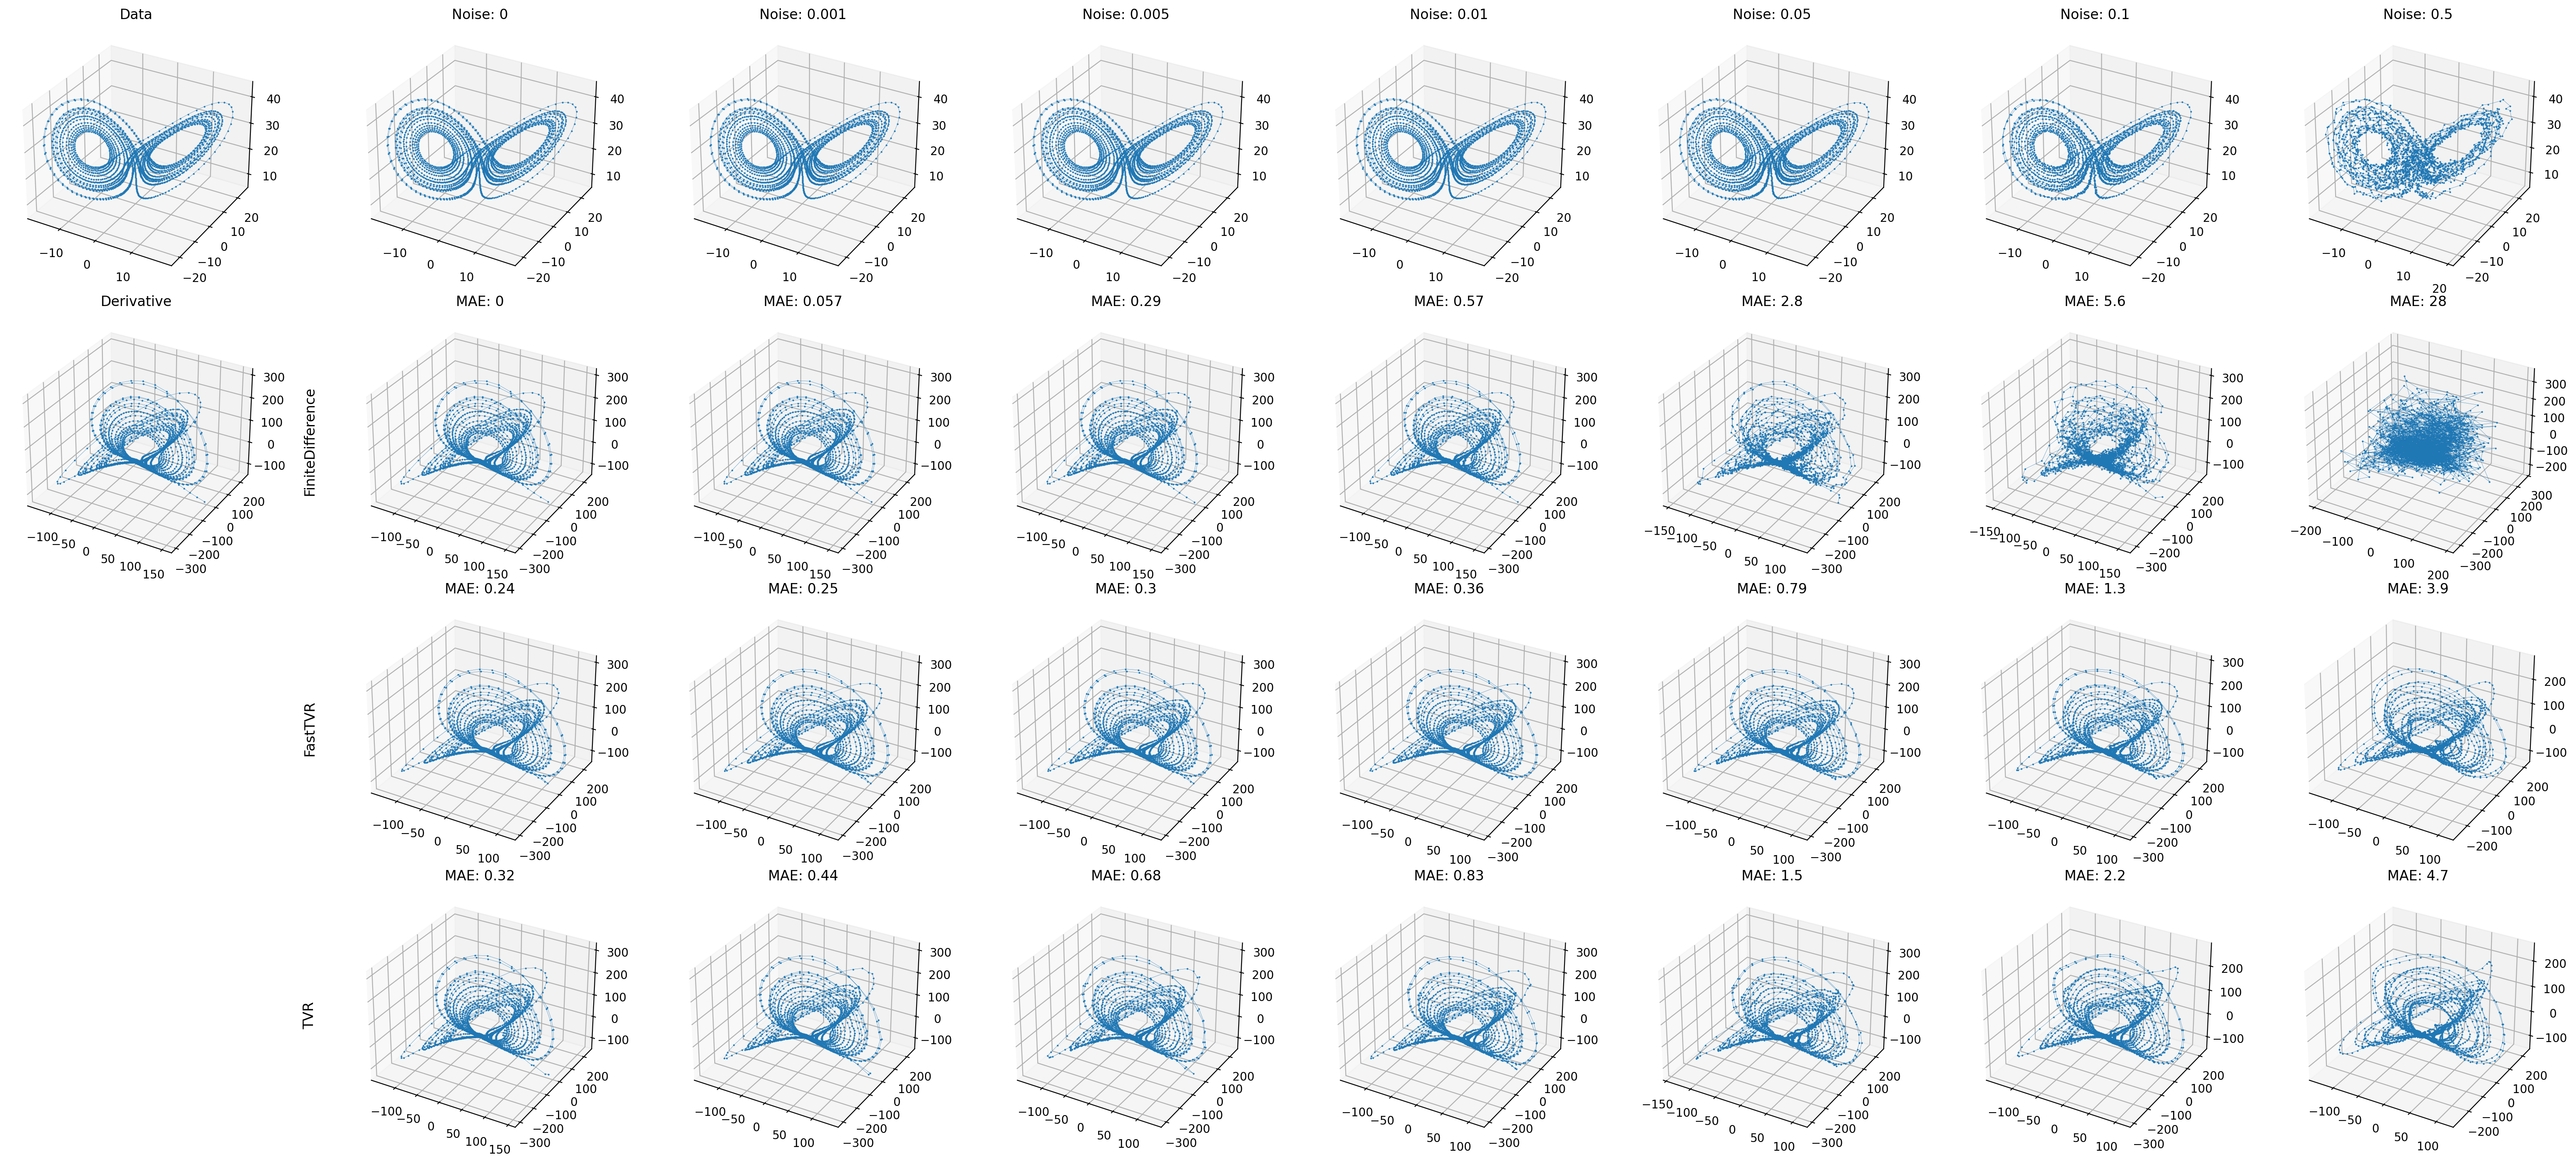
\includegraphics[width=\textwidth]{dif/lorenz_test}
\caption{Дифференцирование данных с различным уровнем шума}
\label{fig:dif:lorenz_test}
\end{figure}

\paragraph{Общие выводы}

По результатам тестирования можно сказать, что успешно дифференцировать зашумленные данные вполне реально. Анализ результатов позволяет сделать некоторое выводы о подборе параметров.

Во-первых, чем больше измерений значений функции в единицу времени дано, тем точнее будет полученная производная. Изменение шага сетки является способом контроля погрешности еще в методе конечных разностей и здесь не теряет свою актуальность. Во-вторых, для итеративного метода дифференцирования оптимальным числом итераций является 2. После первой итерации производная еще не достаточно приняла свою форму, а после третьей и далее она становится слишком ступенчатой. Наконец, более подробно остановимся на коэффициенте регуляризации --- параметре, имеющемся у обоих методов.

Из графиков видно, что порядок коэффициента приблизительно линейно связан с порядком уровня шума. Это подтверждает и рисунок~\ref{fig:dif:alpha_test}, на котором изображены оптимальные траектории параметра $\alpha$ в зависимости от уровня шума для нескольких тестируемых функций (в основном систем ОДУ, которые будут использованы в следующем пункте), серой пунктирной линией изображен примерный тренд.

\begin{figure}
\begin{subfigure}[t]{0.9\linewidth}
	\centering
	\includegraphics[width=\linewidth]{dif/alpha_fast_tvr}
	\caption{}
\end{subfigure}

\begin{subfigure}[t]{0.9\linewidth}
	\centering
	\includegraphics[width=\linewidth]{dif/alpha_tvr}
	\caption{}
\end{subfigure}
\caption{Оптимальные значения параметра $\alpha$: a) для первого метода; б) для второго метода}
\label{fig:dif:alpha_test}
\end{figure}

При этом для различных функций порядок параметра может сильно различаться. В целом возникает субъективное ощущение, что чем \enquote{сложнее} функция (с точками разрыва или просто более извилистая), тем меньше должен быть коэффициент регуляризации.

\paragraph{Замер времени}

Как было сказано в описании разработки~\ref{section:practice}, оба метода реализованы с явным использованием матричных операторов дифференцирования и интегрирования. Поэтому от них можно ожидать полиномиальной сложности от квадратичной и выше. На рисунке~\ref{fig:dif:time} изображена зависимость времени дифференцирования от числа замеров в единицу времени (измерения проводились на процессоре \texttt{AMD Ryzen 7 3700U}). Действительно, при увеличении числа замеров на порядок, затраченное время увеличивается примерно на два порядка.

\begin{figure}
\includegraphics[width=0.9\textwidth]{dif/time}
\caption{Зависимость времени дифференцирования от количества данных}
\label{fig:dif:time}
\end{figure}
